\documentclass[11pt]{article}
\title{\textbf{Horns unit}}
\author{https://github.com/heptagons/meccano/units/horns}
\date{}

\usepackage{../../meccano}
\usepackage{tikz}
\usetikzlibrary{calc}

\begin{document}

\maketitle
\begin{abstract}
Horns unit is a group of seven meccano\meccanoref strips intended to build polygons.
\end{abstract}

\begin{figure}[h]
\centering
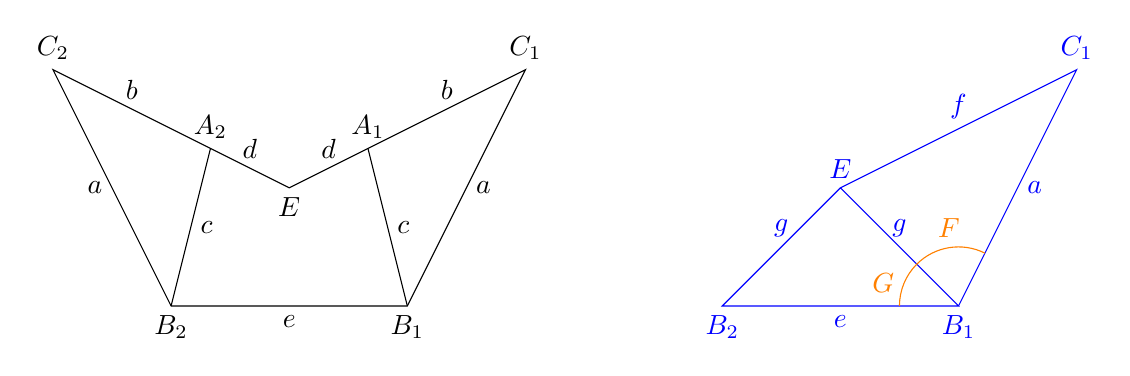
\begin{tikzpicture}
 \begin{scope}[scale=0.5]
  \draw[black] (0,0)
  -- node[below] {$e$} ++(6,0) node[below] {$B_1$}
  -- node[below,right] {$a$} ++(3,6) node[above] {$C_1$}
  -- node[above] {$b$} ++(-4,-2) node[above] {$A_1$}
  -- node[above] {$d$} ++(-2,-1) node[below] {$E$}
  -- node[above] {$d$} ++(-2,1) node[above] {$A_2$}
  -- node[above] {$b$} ++(-4,2) node[above] {$C_2$}
  -- node[below,left] {$a$} ++(3,-6) node[below] {$B_2$}
  -- cycle;
  \draw[black] (6,0) --++ (-1,4) node[midway,right] {$c$};
  \draw[black] (0,0) --++ (+1,4) node[midway,right] {$c$};

  \draw[blue] (20,0)
  -- node[below,right] {$a$} ++(3,6) node[above] {$C_1$}
  -- node[above] {$f$} ++(-6,-3) node[above] {$E$}
  -- node[above] {$g$} ++(-3,-3) node[below] {$B_2$}
  -- node[below] {$e$} ++(6,0) node[below] {$B_1$}
  -- node[above] {$g$} ++(-3,+3);
  
  \draw[orange] (20,0)+(-1.5,0) 
   arc (180:135:1.5) node[midway,above,left] {$G$}
   arc (135:atan(2):1.5) node[midway,above] {$F$};
 \end{scope}

\end{tikzpicture}
\caption{The \textbf{horn unit} has seven strips: Two of length $a$, two of length $b+d$,
two of length $c$ and one of length $e$.
We expect to build polygons with internal angle $C_1B_1B_2$
and perimeter including segments $a,e,a$.}
\label{fig:horns}
\end{figure}

\section{Algebra}
From figure \ref{fig:horns} we start with triangle $\triangle{A_1B_1C1}$.
At vertex $A_1$ we have angle $A$ and the supplement $A'$:
\begin{align}
A &\equiv \angle{B_1A_1C_1}\\
\cos{A} &= \frac{b^2 + c^2 - a^2}{2bc} &\text{if and only if } a < b+c\\
A' &\equiv \angle{EA_1B_1} = \pi - A\\
\cos{A'} &= \cos{(\pi-A)} = -\cos{A} = \frac{- b^2 - c^2 + a^2}{2bc}
\end{align}

We define $f\equiv b+d$ and $g \equiv \overline{EB_1}$. With the law of cosines we have:
\begin{align}
f &\equiv \boxed{b + d} &\in \bbb{N}\\
g^2 &= c^2 + d^2 - 2cd\cos{A'}\\
 &= c^2 + d^2 - (2cd)\frac{-b^2 - c^2 + a^2}{2bc} \nonumber\\
 &= \frac{bc^2 + bd^2 + b^2d + c^2d - a^2d}{b} \nonumber\\
 &= \frac{(b+d)(bd+c^2) - a^2d }{b}
\end{align}

Define a new variable $h = (b+d)(bd+c^2) - a^2d$:
\begin{align}
h &\equiv \boxed{(bd+c^2)f - a^2d} &\in \bbb{Z}\\
g^2 &= \boxed{\frac{h}{b}}  &\text{if and only if } 0 < h < b
\end{align}


We calculate angles $F \equiv \angle{C_1B1E}$ and $G \equiv \angle{B_2B_1E}$.
We replace $g^2$ by $h/b$:
\begin{align}
\cos{F} &= \frac{a^2 + g^2 - f^2}{2ag} = \frac{a^2b - bf^2 + h}{2abg}\\
\cos{G} &= \boxed{ \frac{e}{2g} }
\end{align}
Define new variable $j = a^2b - bf^2 + h$ so:
\begin{align}
j &\equiv \boxed{a^2b - bf^2 + h} &\in \bbb{Z}\\
\cos{F} &= \frac{a^2b - bf^2 + h}{2abg} = \boxed{\frac{j}{2abg}}
\end{align}

We calculate cosines squares and products. Again we replace $g^2$ by $h/b$:
\begin{align}
\cos{F}\cos{G} &= \frac{ej}{4abg^2} = \frac{bej}{4abh} = \boxed{\frac{ej}{4ah}} &\in \bbb{Q}\\
\cos^2{F} &= \frac{j^2}{4a^2b^2g^2} = \frac{bj^2}{4a^2b^2h} = \boxed{\frac{j^2}{4a^2bh}} &\in \bbb{Q}\\
\cos^2{G} &= \frac{e^2}{4g^2} = \boxed{\frac{be^2}{4h}} &\in \bbb{Q}\\
\cos^2{F}\cos^2{G} &= \frac{be^2j^2}{16a^2bh^2} = \boxed{\frac{e^2j^2}{16a^2h^2}} &\in \bbb{Q}\\
\end{align}

We calculate the sines part squared and set a common denominator as square $16a^2b^2h^2$:
\begin{align}
(\sin{F}\sin{G})^2 &= (1 - cos^2{F})(1 - cos^2{G})\\
 &= 1 - cos^2{F} - cos^2{G} + cos^2{F}\cos^2{G} \nonumber\\
 &= 1 - \frac{j^2}{4a^2bh} - \frac{be^2}{4h} + \frac{e^2j^2}{16a^2h^2}\nonumber\\
 &= 1 - \frac{j^2}{4a^2bh} - \frac{be^2}{4h} + \frac{e^2j^2}{16a^2h^2}\nonumber\\
 &= \frac{16a^2b^2h^2 -(4bh)j^2 -(4a^2b^2h)be^2 +(b^2)e^2j^2 }{16a^2b^2h^2}\nonumber\\
 &= \frac{16a^2b^2h^2 -4bhj^2 -4a^2b^3e^2h +b^2e^2j^2 }{16a^2b^2h^2}\nonumber\\
 &= \frac{b(be^2-4h)(j^2-4a^2bh)}{16a^2b^2h^2}
\end{align}

Extract square root to get $\sin{F}\sin{G} = \sqrt{D}/A$ where $D,A \in \bbb{Z}$:
\begin{align}
\sin{F}\sin{G} &= \boxed{\frac{\sqrt{b(be^2-4h)(j^2-4a^2bh)}}{4abh}} &\in \bbb{A}
\end{align}

We sum the angles $F$ and $G$ to get:
\begin{align}
F+G &\equiv \angle{B_2B_1C_1}\\
\cos{(F+G)} &= \cos{F}\cos{G} - \sin{F}\sin{G}\\
 &= \frac{ej}{4ah} - \frac{\sqrt{b(be^2-4h)(j^2-4a^2bh)}}{4abh}\nonumber\\
 &= \frac{bej - \sqrt{b(be^2-4h)(j^2-4a^2bh)}}{4abh} &\in \bbb{A}
\end{align}

\section{Software}

\section{Examples}

\newcommand{\horns}[8]{ % size,factor,a,b,c,d,e,ang
 \begin{tikzpicture}
 \def\a{#3};\def\b{#4};\def\c{#5};\def\d{#6};\def\e{#7};\def\ang{#8}
 \pgfmathsetmacro\f{#4+#6}
 \pgfmathsetmacro\angB{(pow(#3,2) + pow(#5,2) - pow(#4,2))/(2*#3*#5)} % aa+cc-bb/2ac
 \pgfmathsetmacro\angC{(pow(#3,2) + pow(#4,2) - pow(#5,2))/(2*#3*#4)} % aa+bb-cc/2ab
 \begin{scope}
  \meccanostrip[FF0000]{#7}{#1}{#2} %e
 \end{scope}
 \begin{scope}[shift={(#1*#7,0)},rotate=\ang]
  \meccanostrip[008800]{#7}{#1}{#2} %a long as e right
  \begin{scope}[rotate=acos(\angB)]
   \meccanostrip[0000FF]{#5}{#1}{#2} %c
  \end{scope}
  \begin{scope}[shift={(#1*#3,0)},rotate=180-acos(\angC)] % a
   \meccanostrip[cc00cc]{\f}{#1}{#2} %b+d=f
  \end{scope}
 \end{scope}
 \begin{scope}[rotate=180-\ang]
  \meccanostrip[008800]{#7}{#1}{#2} %a long as e left
  \begin{scope}[rotate=-acos(\angB)]
   \meccanostrip[0000FF]{\c}{#1}{#2} %c
  \end{scope}
  \begin{scope}[shift={(#1*\a,0)},rotate=180+acos(\angC)]
   \meccanostrip[cc00cc]{\f}{#1}{#2} %b+d=f
  \end{scope}
 \end{scope}
 \end{tikzpicture}
}

\subsection{Octagons examples}

\begin{figure}[H]
\centering
\scalebox{0.5}{ \horns{1}{5pt}{2}{3}{3}{3}{8}{45}}
\caption{Horns(2,3,3,3,8) $45^\circ$.}
\end{figure}

\begin{figure}[H]
\centering
\scalebox{0.45}{ \horns{1}{5pt}{3}{2}{3}{7}{12}{45}}
\caption{Horns(3,2,3,7,12) $45^\circ$.}
\end{figure}

\begin{figure}[H]
\centering
\scalebox{0.3}{\horns{1}{5pt}{14}{9}{9}{9}{16}{45}}
\caption{Horns(14,9,9,9,16) $45^\circ$.}
\end{figure}

\begin{figure}[H]
\centering
\scalebox{0.25}{\horns{1}{5pt}{14}{11}{11}{11}{24}{45}}
\caption{Horns(14,11,11,11,24) $45^\circ$.}
\end{figure}

\begin{figure}[H]
\centering
\scalebox{0.25}{\horns{1}{5pt}{21}{21}{14}{6}{24}{45}}
\caption{Horns(21,21,14,6,24) $45^\circ$.}
\end{figure}

\end{document}
